\documentclass[11pt,a4paper]{report}
\usepackage[utf8x]{inputenc}
\usepackage{graphicx}
\usepackage[labelfont=bf]{caption}
\usepackage{float}
\usepackage{hyperref}
\usepackage{amsmath}

% Windows
%\graphicspath{{C:/Users/achantreau/Documents/GitHub/BEng-Individual-Project/Report/images/}}

% Linux
\graphicspath{{/homes/ac6609/Documents/BEng-Individual-Project/Report/images/}}

\usepackage{fancyhdr}
\setlength{\headheight}{30pt}
\pagestyle{fancy}

\renewcommand{\chaptermark}[1]{\markboth{#1}{}}
\renewcommand{\sectionmark}[1]{\markright{#1}{}}

\fancyhf{}
\lhead{\fancyplain{}{\thepage}}
\chead{}
\rhead{\fancyplain{}{\textit{\leftmark}}}
\rfoot{\thepage}

\setlength\parindent{0pt}
\setcounter{page}{1}
\pagenumbering{roman}

\newcommand{\HRule}{\rule{\linewidth}{0.5mm}}
\newcommand{\me}{\mathrm{e}}

%\numberwithin{equation}{section}

\begin{document}

%-----------------------------------------------------------
% TITLE SECTION
%-----------------------------------------------------------
\begin{titlepage}
\begin{center}

\textsc{\LARGE Imperial College London}\\[1.5cm]

\textsc{\Large BEng Individual Project - Final Report}\\[0.5cm]

% Title
\HRule \\[0.4cm]
{ \huge \bfseries jSCAPE - Java Self-assessment Center of Adaptive Programming Exercises \\[0.4cm] }

\HRule \\[1.5cm]

% Author and supervisor
\begin{minipage}{0.4\textwidth}
\begin{flushleft} \large
\emph{Author:}\\
Alexis \textsc{Chantreau}
\end{flushleft}
\end{minipage}
\begin{minipage}{0.4\textwidth}
\begin{flushright} \large
\emph{Supervisor:} \\
Dr.~Tristan \textsc{Allwood}
\end{flushright}
\end{minipage}

\vfill

% Bottom of the page
{\large \today}

\end{center}
\end{titlepage}

%-----------------------------------------------------------
% ABSTRACT SECTION
%-----------------------------------------------------------
%\begin{abstract}\centering
%
%\end{abstract}

%-----------------------------------------------------------
% TABLE OF CONTENTS SECTION
%-----------------------------------------------------------
\tableofcontents

\newpage
\setcounter{page}{1}
\pagenumbering{arabic}

%-----------------------------------------------------------
% LIST OF FIGURES SECTION
%-----------------------------------------------------------
\listoffigures

%-----------------------------------------------------------
% INTRODUCTION SECTION
%-----------------------------------------------------------
\chapter{Introduction}

\section{Motivation}
Programming is generally acknowledged to be a difficult discipline to learn, requiring problem solving skills, attention to detail and the ability to think abstractly. One could say that these skills are somewhat developed in high school during mathematics courses, but programming is still a ``beast" of its own. In addition, different programming paradigms exist, such as functional programming or imperative programming. Knowing how to program in Java can still make learning Haskell a difficult process.\newline

Yet, in this 21st century society, programming is definitely a useful skill to have, and there is an interest in the population to learn these skills. Indeed, this can be seen by the number of students enrolling in computer science courses at universities, or the increase in websites such as Codecademy\cite{Codecademy}, Coursera\cite{Coursera}, Udacity\cite{Udacity}, which provide online computer science/programming courses for free.\newline

In many of these situations, it is difficult for teachers, lecturers or course leaders to provide enough support through exercises, assignments and to monitor student's progress in such a way which allows them to modify their teaching to help struggling students. Indeed, teachers and students can generally only rely on a few homework assignments to get an idea of how they are doing. Coming up with a solution to increase the amount of practise and feedback would be beneficial to both students and teachers. \newline

Thus, there is a clear need to provide a platform for students to practise their programming skills and understanding of programming concepts, in a context of self-assessment only. In such a system, requiring teachers to come up with all the exercises by themselves can be both time consuming and ineffective: some exercises may not be challenging enough for certain top students, or on the contrary too difficult for struggling students, which can be discouraging for them.

\section{Objectives}
Having identified the problems associated with teaching and learning programming, we were led to formulating objectives in order to make the project successful and useful to the parties involved. \newline

The main objective of the project was to produce a web-based application to be used in self-assessing one's programming knowledge, whether it be in high school, at university or as part of an online course. For this application, four key features were identified:

\begin{itemize}
\item \textbf{Programming questions/exercises -} The web platform should allow students to practise their programming skills and understanding of programming concepts. There should be no limit to the number of questions a student can answer, so that if a student desires more practice, then he should be able to do that. Additionally, it should be possible for a specific set of people, such as teachers, lecturers or tutors, to add questions/exercises to the system.
\item \textbf{Progress tracking -} Designated people, such as teachers, lecturers or tutors, should have access to detailed statistics about the students performances. This will provide them with useful information about difficulties particular students, or the entire class, may be facing. In addition, the system should give feedback to the students, in the form of simple statistics, allowing them to identify their weak areas and thus improve on them.
\item \textbf{Adaptive difficulty -} The questions or exercises presented to the students should be suited to their ability. Not only will this stimulate the learning process, but it will also give a better indication of a student's understanding of the programming concepts being tested.
\item \textbf{Automated generation -} There should be a mechanism to allow for some degree of automated or semi-automated generation of exercises. This will provide a large supply of ``fresh" questions, so that students don't end up answering the same questions and memorizing the answers to them.
\end{itemize}

While investigating existing solutions (chapter \ref{chap:related-work}) we found out that some of these features were less common than others. The availability of programming exercises and progress tracking are very essential in such systems, therefore many of the related software we looked at implemented these features. On the other hand, relatively few tools integrated some form of adaptive difficulty. Finally, almost none of the tools featured automated generation of questions, opting instead to allow exercises to be added manually to the system, or downloaded from existing exercise banks.

\section{Contributions}
Within the context given above, this project makes the following contributions:
\begin{itemize}
\item \textbf{jSCAPE}: a web application for students, named Java Self-assessment Center of Adaptive Programming Exercises, with the following features:
      \begin{itemize}
      \item[-] the ability to view programming exercises and answer them while receiving feedback, a so called form of self-assessment.
      \item[-] graphs, tables and pie charts displaying statistical data on the student's performance.
      \item[-] three different exercise selection algorithms, that decide which is the best exercise to present to the student.
      \end{itemize}
\item \textbf{Admin tool}: a tool for teachers/lecturers/tutors for:
      \begin{itemize}
      \item[-] displaying student performance statistics.
      \item[-] displaying exercise statistics.
      \item[-] defining exercise categories.
      \item[-] adding exercises manually.
      \item[-] generating exercises automatically.
      \end{itemize}
\end{itemize}

\section{Report Structure}
Chapter \ref{chap:background} will present the theoretical basis for this project and the concepts necessary to follow the implementation details of the system.\newline

Chapter \ref{chap:related-work} will give an overview of related work, and will mention how these influenced the design of jSCAPE, in particular which features would be useful for such as system.\newline

Chapter \ref{chap:jscape-system} will present the jSCAPE system in detail, showing all the features which are available.\newline

Chapter \ref{chap:implementation} will cover the design and implementation details of the jSCAPE system, in particular how the difficulty of exercises is adapted to the student's ability and how exercises can be automatically generated.\newline

Chapter \ref{chap:evaluation} will contain the results of evaluating jSCAPE as a whole, and its different components. \newline

Chapter \ref{chap:conclusion} summarises the achievements of the project and discusses possible extensions that can be made to the system in the future.


%-----------------------------------------------------------
% BACKGROUND SECTION
%-----------------------------------------------------------
\chapter{Background}
% Add maximum likelihood background explanation
% Add Bayesian probability background explanation
%Add note to say that we use the word examinee to mean someone taking a test although the test may not be an exam per say.

\section{Computer Based Tests}
CBT abbreviation
- offers advantages such as being able to display higher quality visuals such as pictures, videos, graphs, etc...
- low paperwork, everything is stored on the computer
- automatic grading, less work for teachers
- generation of statistics is made easier by the fact that the data can be processed by the computer
- nowadays a lot of learning is done on computer systems, and children are used to dealing with computers so assessment through this medium is advantageous. \newline

CBTs are typically "fixed-item" tests where all the students answer the same set of questions,  usually provided by the person responsible for the assessment. This isn't ideal since students can be presented with questions that are too easy or too difficult for them to answer. Consequently, the results of the test won't give a very accurate representation of a student's ability, and for this reason, these types of tests aren't extremely useful. This problem lead to research and the development of computerized adaptive testing (CAT).

\section{Computerized Adaptive Testing}
\label{sec:CAT}
Computerized adaptive testing (CAT), also called \textit{tailored testing}, is a form of computer-based testing which administers questions (referred to as \textit{items} in the psychometrics literature) of the appropriate difficulty by adapting to the examinee's ability.
For example, if an examinee answers an item correctly, then the next item presented will higher on the difficulty scale. On the other hand, if they answer incorrectly, they will be presented with an item lower on the difficulty scale. \newline

From an architectural perspective, a computerized adaptive test (CAT) consists of five components \cite{CAT-Framework}:

\subsubsection{1. Calibrated item pool}
An item pool is needed to store all the items available for inclusion in a test. This item pool must be calibrated with a psychometric model. During this phase, the item parameters are estimated according to the chosen model and scaled to fit with already existing items. Usually, the psychometric model employed in these systems is called Item Response Theory (IRT) (section \ref{subsec:IRT}). Calibration is a complex process, and to be done accurately it requires a considerable amount of data. Typically, it is performed by psychometricians, aided by expensive and sophisticated calibration software.

\subsubsection{2. Starting point}
Initially, when zero items have been administered, no information is known about the examinees and so the CAT is unable to estimate their ability. As a result, the item selection algorithm will fail to choose the next item to be administered.
If there is previous information available, for example an examinee's ability estimate in a closely related subject, then this can be input into the system to form the starting point configuration. Often this data isn't available or too costly to collect, so the CAT's initial ability estimate for the examinee corresponds to the mean on the ability scale - hence the first item presented will be of average difficulty.

\subsubsection{3. Item selection algorithm}
The item selection algorithm chooses the next item to present to the examinee based on the ability estimate of the examinee up to that point. Several methods exist and largely depend on the psychometric model in use. One of the most commonly used methods is the \textit{maximum information method} (section \ref{subsec:IRT}), which selects the item which maximizes the information function with respect to the estimated ability at that point.

\subsubsection{4. Scoring algorithm}
The scoring algorithm refers to the steps taken to update the examinee's ability estimate after an item has been answered. The two most commonly used methods are \textit{maximum likelihood estimation} (section \ref{subsec:IRT}) and \textit{Bayesian estimation} (section \ref{subsec:IRT}).

\subsubsection{5. Termination criterion}
The termination criterion specifies when the CAT should finish. For example the CAT can terminate when the change in the ability estimate after each iteration is below a certain threshold, or when time has run out, or when $N$ items have been administered, etc... Obviously, the CAT shouldn't be terminated too early, so as to allow enough time to estimate the examinee's ability with acceptable accuracy.

\begin{figure}[H]
\centering
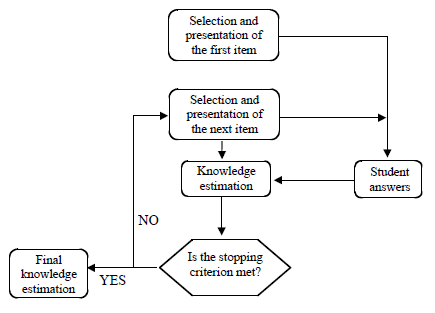
\includegraphics[scale=1]{cat_flowchart}
\caption{Flowchart of an adaptive test. Adapted from \cite{SIETTE}.}
\label{fig:cat_flowchart}
\end{figure}

The flowchart in figure~\ref{fig:cat_flowchart} corresponds to components 2-5, and illustrates the basics of the algorithm implemented in CAT. \cite{CAT-Wiki} gives a more detailed description of the procedure:
\begin{itemize}
\item[1.] The pool of items that haven't been administered yet is searched to determine the best item to present to the examinee, according to the current estimation of his ability.
\item[2.] The chosen item is presented to the examinee, who then answers it correctly or incorrectly.
\item[3.] The ability estimate is updated, based upon this new piece of information and the previous ability estimate.
\item[4.] Steps 1–3 are repeated until a termination criterion is met.
\item[5.] The algorithm returns a final ability estimate for the examinee's performance along with a confidence level: a percentage value indicating how accurate the estimate is.
\end{itemize}

CATs offer several advantages over traditional CBTs. As a result CATs have been used in many areas\cite{CAT-Areas}, such as education, job hiring, counselling, clinical studies, etc... Since CATs administer items by adapting to the examinee's ability, the test-taking experience ends up being a more positive one. Indeed, examinees won't have to deal with answering items which are too difficult or too easy compared to their ability level, a problem which appears in traditional CBTs.\newline

In addition, by administering only those items which will yield additional information, CATs end up being more accurate in estimating an examinee's ability level. This contrasts with CBTs which usually provide the best precision for examinees of medium ability, whereas extreme scores end up being less accurate.\newline

Lastly, CATs can come up with an ability estimate much quicker and with fewer administered items when compared to traditional CBTs. Indeed, an adaptive test can typically be shortened by 50\% and still maintain a higher level of precision than a fixed version.\cite{Weiss1984}
\newline

Despite the advantages mentioned above, CATs have some limitations. A frequent complaint is that an examinee isn't allowed to go back and change his answer to a past item. This limitation exists to prevent the examinee from intentionally answering items incorrectly to make subsequent items easier, and then going back and selecting the correct answers to achieve a perfect score. For similar reasons, it isn't possible to skip items, the examinee must select an answer to move on to the next item.\newline

The second issue has to do with the items themselves. First of all, there is the need for a large bank of items to cater to all ability levels. Developing an item pool of sufficient size can be very time consuming. David J. Weiss writes in \cite{Weiss1985} that item pools with 150-200 items are to be preferred, although 100 high quality items can sometimes be enough to achieve adequate estimations of ability levels.

Secondly, for the CAT to be of good quality the item pool needs to be calibrated accurately. This requires pre-administering the items to a sizeable sample and then simultaneously estimating all the item parameters for each item. The guidelines in \cite{CAT-Primer} suggest that sample sizes may be as large as $1000$ examinees. This phase is costly, time consuming and often times simply unfeasible.\newline

Lastly, item exposure is a possible security concern. Sometimes particular items may be presented too often and become overused. This may result in examinees becoming familiar with them and sharing them to other examinees of the same ability level, thus corrupting the results of the test. This problem can be solved to some extent by modifying the item selection algorithm to include some exposure control mechanism.\newline

A brief overview of CATs was given in this section. All of these concepts will be explored in more detail in item response theory (section \ref{subsec:IRT}) and in the implementation of adaptive testing in jSCAPE (chapter XX?).

\section{Probabilistic Test Theory}
In this section we go over a few topics in probability and how they can be implemented successfully in the area of computer assessments.

\subsection{Likelihood and Maximum Likelihood Estimation}
Although the terms probability and likelihood are used interchangeably in every day life, in statistics a distinction can be made.\newline

For any stochastic process, let us denote the observed outcomes as $x$ and the set of parameters as $\theta$. When we say probability, we want to calculate $P(x | \theta)$, i.e. the probability of observing the outcomes $x$ given specific values for the set of parameters $\theta$. \newline



In more mathematical terms, we have:
$$L(\theta | x) = P(x | \theta)$$

To highlight the distinction we illustrate with an example of how the two terms are used. If we consider a dice, a possible parameter is the fairness of the dice, while possible outcomes are which values are displayed after a roll. For instance, if a fair dice is rolled 5 times, what is the \textit{probability} that a 6 will show up on every roll? If a dice is rolled 5 times and lands on 6 every roll, what is the \textit{likelihood} that the dice is fair? \newline

Maximum likelihood estimation refers to a method of statistical inference where one can find the set of parameter values ($\theta$) which are most \textit{likely} given the observed outcomes ($x$). As mentioned in the name of the method, this is done by finding the parameter values which maximize the likelihood function $L(\theta | x)$.

\subsection{Bayes probability theory}
% Add maximum likelihood background explanation
% Conditional probability quick overview?
% Add Bayesian probability background explanation
% Bayesian networks
% Latent variables ?

\subsection{Item Response Theory}
\label{subsec:IRT}
We mentioned in section \ref{sec:CAT} that Item Response Theory (IRT) is usually the psychometric model of choice when developing a CAT, e.g. the Graduate Record Examination (GRE) and Graduate Management Admission Test (GMAT). CATs can still be implemented with Classical Test Theory but they offer less sophistication and less information to evaluate/improve the reliability of the test, making IRT the superior choice. \newline

IRT attempts to model the answer to an item as a mathematical model. \newline

Several IRT models have been developed over the years to address the different types of tests that exist, e.g. multiple choice exams, agreement questionnaires (Likert scale), etc... These models all seek to achieve the same goal, modelling the examinee's ability on some ability scale, but they differ in the number of parameters associated with each item. We now take a greater look at these different models:

\subsubsection{The one-parameter logistic model}
\begin{equation} \label{eq:1PL-IRF}
P(\theta) = \frac{1}{1 + \me^{-(\theta - b)}}
\end{equation}

Equation \eqref{eq:1PL-IRF} shows the item response function for the one-parameter logistic model (1PL). 

\subsubsection{The two-parameter logistic model}
\begin{equation} \label{eq:2PL-IRF}
P(\theta) = \frac{1}{1 + \me^{-1.7a(\theta - b)}}
\end{equation}

Equation \eqref{eq:2PL-IRF} shows the item response function for the two-parameter logistic model (2PL). 

\subsubsection{The three-parameter logistic model}
\begin{equation} \label{eq:3PL-IRF}
P(\theta) = c + \frac{1 - c}{1 + \me^{-1.7a(\theta - b)}}
\end{equation}

Equation \eqref{eq:3PL-IRF} shows the item response function for the three-parameter logistic model (3PL). 

\subsubsection{Estimating the ability}
In section \ref{sec:CAT}, when discussing scoring algorithms, we saw that the two most common methods for ability estimation were \textit{maximum likelihood estimation} and \textit{Bayesian estimation}.\newline

In the \textit{maximum likelihood estimation} method, we need to define a likelihood function in terms of the ability level ($\theta$) we are trying to estimate:

\begin{equation} \label{eq:Trait-estimation}
L(\theta | \textbf{u}) = L(\theta | u_1, ..., u_n) = P(u_1, ..., u_n | \theta) = \prod_{i=1}^n P_i(\theta)^{u_i}(1 - P_i(\theta))^{(1 - u_i)} ,
\end{equation}

where $\textbf{u}=(u_1, ..., u_n)$ is called the reponse vector for an examinee, that is $u_i=1$ if the examinee answers the i$^\text{th}$ item correctly, and $u_i=0$ if the examinee answers the i$^\text{th}$ item incorrectly. $P_i(\theta)$ corresponds to the probability of answering the i$^\text{th}$ item correctly when the ability level is $\theta$, and thus $1 - P_i(\theta)$ gives the probability of answering the i$^\text{th}$ item incorrectly when the ability level is $\theta$. \newline

Now that the likelihood function is defined, we can apply maximum likelihood estimation to find the ability level which is most likely given the examinee's response vector. Let us illustrate with a very simplistic example where ability levels are discrete values between $-1$ and $+1$. We would iterate through these ability levels and compute the following values, for example:
\begin{align*}
L(\theta=-1 | \textbf{u}) &= 0.001 \\
L(\theta=+0 | \textbf{u}) &= 0.012 \\
L(\theta=+1 | \textbf{u}) &= 0.054
\end{align*}

The likelihood function is maximized when $\theta = +1$, and so this is the maximum likelihood estimate for $\theta$. In a CAT, and based on the examinee's response vector \textbf{u}, the system would assign $+1$ as the ability level for that examinee.\newline

The \textit{Bayesian estimation} method is also somewhat based on the likelihood function and therefore very similar to \textit{maximum likelihood estimation}.........


\subsubsection{Item information}

\section{Summary}
We have gone over types of computer based assessment and how they differ from regular assessment techniques. We have also provided an overview of the theoretical components and probability concepts which will be implemented in jSCAPE (chapter xx?).


%-----------------------------------------------------------
% RELATED WORK SECTION
%-----------------------------------------------------------
\chapter{Related Work}
\label{chap:related-work}
With the rise of computer usage in today's society, they have quite naturally made their way over to education. As such, web-based, computer-based and adaptive assessment systems have been investigated and researched quite thoroughly over the years. The result of this research is numerous tools and software which provide students the opportunity to practise their programming skills, whether it be by writing code or answering programming questions, in an environment which tracks their progress. Almost all of these tools provide the basic features, that is the programming exercises themselves, and a component to view statistics or student results. Some of them distinguish themselves by adding useful and not so common features such as adaptive difficulty. From all the solutions we looked at, very few provided automate exercise generation, and for those who did, their approach was only limited to extremely simple exercises. \newline

We have looked at quite a few solutions such as ELP (Environment for Learning to Program) and CourseMaster, which have the very basic features. We do not go into detail about how these solutions operate since the details are quite straightfowrad and not very interesting. Instead we focus on software which has approached the adaptive difficulty problem, and look into how they did so.\newline

In this section we look at the related software which has influenced the design and implementation of our proposed solution, jSCAPE.

\section{Programming Adaptive Testing}
\label{sec:PAT}
PAT\cite{PAT} is a web-based adaptive testing system, developed in ActionScript/Flash, for assessing students' programming knowledge in Greek high schools. \newline

The assessment is carried out by presenting students with 30 questions from various chapters of the introductory programming course. Some of the questions supported by the PAT system are true/false questions, multiple choice questions, gap filling in a piece of code, questions involving diagrams and questions where one has to determine the behaviour of a piece of code.\newline

In PAT, questions are classified into different difficulty categories. Category A is for easy questions, category B is for intermediate questions and category C is for difficult questions. PAT seeks to adapt the difficulty of the questions to the student's ability, by choosing questions of the appropriate difficulty category.

\begin{figure}[H]
\centering
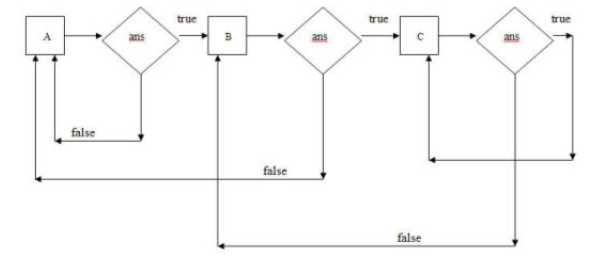
\includegraphics[width=\textwidth,height=\textheight,keepaspectratio]{PAT_adaptive_sequence}
\caption{Adaptive sequence of questions in PAT. (Source:\cite{PAT})}
\label{fig:PAT_adaptive_sequence}
\end{figure}

Figure \ref{fig:PAT_adaptive_sequence} shows the possible adaptive sequences. This algorithm is quite simplistic, every correct answer leads to a promotion to the next level of difficulty until no further promotions are possible. Likewise, every incorrect answer leads to a demotion to a lower level of difficulty until no further demotions are possible.\newline

At the end of the test, the system shows the student's total number of correct answers out of 30 and how well the student performed on each chapter. Also, PAT classifies the student into one of three programming skill levels based on their final score and a weighted score, where the difficulty of the questions answered correctly is considered. These results are available to both students and teachers so that they can be used to improve performance later on in the school year.\newline

We feel that the adaptive algorithm increases the difficulty of questions too quickly and doesn't take into account guessing or possible slip ups from students. This limitation can be circumvented by, for instance, requiring a number of correct answers at the current difficulty level before progressing to the next one.\newline

PAT only provides assessment at specific times throughout the school year and no opportunity for students to practice and self-assess in their own time. In addition, it isn't possible for teachers to upload their own questions to the system. The question bank remains static and contains 443 questions. Lastly, the authors of PAT admit that the statistical data available to students and teachers is fairly limited, and that improvements should be pursued in future work.

\section{SIETTE}
\label{sec:SIETTE}
SIETTE\cite{SIETTE-small} (System of Intelligent Evaluation Using Tests for Tele-education) is a web based environment for generating and constructing adaptive tests. It has been used with great success in courses from the computer science engineering school, the telecommunication engineering school and the philosophy faculty, all at the University of Malaga, Spain.\newline

SIETTE is a vast system, and at the time of publication (2005) it contained information about $15000$ student test sessions, and the knowledge base contained 84 subjects, 1852 topics, 3820 question and 220 tests.\newline

SIETTE is designed to be used by both students and teachers. Teachers use the system to create tests, define the subject topics, the questions and their parameters. Students use the system to take the tests specified by the teachers. The tests can be used for self-assessment, where the correction is shown immediately after the student has answered. Hints and more extensive feedback are also available in this mode. Or, the tests can be used as exams, where the score counts towards the student's final grade. In this mode, hints and feedback aren't provided. It is important to note that tests have a fixed number of questions, thus, new tests must be created every time a student runs out of practice.\newline

As mentioned earlier, SIETTE constructs adaptive tests, therefore, when a student answers a question, his ability is re-estimated and the next question is selected accordingly. Implementation of this is done by using item response theory in the computerized adaptive testing framework.\newline

SIETTE uses the three-parameter logistic (3PL) model and measures the student's knowledge in terms of a discrete random variable $\theta$, which ranges from 0 to $K-1$, where $K$ is the number of discrete knowledge levels. When it comes to creating items, the guessing parameter $c$ is determined automatically, whereas the other two parameters must be entered by the teacher. The discrimination parameter ($a$) must be a number between $0.5$ and $1.5$. The difficulty parameter must be a natural number between 0 and $K-1$. A few years after the SIETTE paper was published, the authors added an item calibration tool because teacher estimates of item parameters are never very accurate.\newline

To estimate students' knowledge level, SIETTE uses the Bayesian estimation method (section \ref{subsec:IRT}) with a knowledge distribution per student, per topic. Also, SIETTE provides teachers with the option of choosing different item selection procedures for tests, such as random selection, difficulty-based selection and bayesian selection.

\begin{figure}[H]
\centering
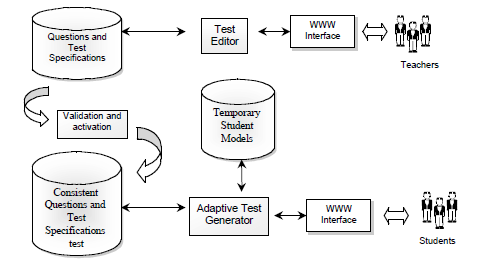
\includegraphics[width=\textwidth,height=\textheight,keepaspectratio]{siette-architecture}
\caption{SIETTE Architecture. (Source:\cite{SIETTE})}
\label{fig:siette-architecture}
\end{figure}

Figure \ref{fig:siette-architecture} gives on overview of the SIETTE architecture. The system is comprised of several components\cite{SIETTE-components}:
\begin{itemize}
\item The \textit{knowledge base}: where tests, topics and questions are stored. Some supported question types are true/false, multiple choice, multiple response and fill-in-the-gap. More interactive questions also exist, implemented as Java applets, where one has to color parts of a map, or move around objects so that they appear chronologically, for example.
\item The \textit{student model repository}: a collection of student models, where information about students' knowledge level estimation, which questions they answered, etc... is stored.
\item The \textit{student workspace}: a web interface where students take tests.
\item The \textit{test editor}: a tool where teachers can define tests, topics, questions.
\item The \textit{result analyzer}: a tool which presents graphical data about students' performance, knowledge estimation levels, etc...
\item The \textit{item calibration tool}: a module used to calibrate items by determining the item parameters (difficulty, discrimination and pseudo-chance).
\end{itemize}

SIETTE is a large and complex system, containing many useful features relevant to the area of web-education, and going through all of these wouldn't be possible. Since SIETTE has been used to such success in university courses we decide to inspire ourselves from this system, especially for the implementation of the adaptive difficulty component. Details about the algorithms used in SIETTE, and hence jSCAPE, can be found in section \ref{sec:implementing-cat}, with Java code to illustrate. However, SIETTE does not provide mechanisms to automatically generate exercises, and so we shall define our own algorithms for this.

\section{Summary}
We have looked at some of the relevant work in the field of computer based education and assessment. We saw that PAT provided a simple algorithm for increasing or decreasing the difficulty of exercises, and so an improved version of this algorithm will feature in jSCAPE. We also saw that SIETTE provided many of the features we set out to replicate in jSCAPE, therefore particular parts of our implementation will be inspired by SIETTE.\newline

SIETTE is the most complete system we have come across while doing research for this project. Moreover, examining some existing solutions which haven't been detailed in this section, has given us insight into the most common features available in these types of systems. \newline

In the next chapter we present the system developed as part of this project: jSCAPE. 

%-----------------------------------------------------------
% PROJECT PLAN SECTION
%-----------------------------------------------------------


%-----------------------------------------------------------
% EVALUATION SECTION
%-----------------------------------------------------------

\chapter{Evaluation}
Mention how our developed system performs against the advantages and disadvantages of CAT.

The evaluation stage will address mostly these two aspects:
\begin{itemize}
\item The system has correctly modelled the ability of students
\item The system is useful in helping students to learn programming and helping lecturers with getting feedback on their teaching, in the form of statistics.
\end{itemize}

\section{Qualitative}
\begin{itemize}
\item Surveys to get feedback from students on interface, usability, etc...
\item 
\end{itemize}

\section{Quantitative}
\begin{itemize}
\item Statistical analysis to evaluate item calibration and modelling of student's abilities
\item 
\end{itemize}

%-----------------------------------------------------------
% CONCLUSION SECTION
%-----------------------------------------------------------
\chapter{Conclusion}
\section{Future Work}
\begin{itemize}
\item Very flexible system so other programming languages could be offered, i.e. cSCAPE, for C and hSCAPE for Haskell. 
\item Working more extensively on the adaptive component of the system, i.e. improving the algorithm which selects questions for students based on their estimated ability.
\item Extend system to allow admins to provide their own question templates, maybe come up with a template grammar which then allows questions to be automatically generated. Or at least allow pluggable function references which will be called to generate the exercise component.
\item Add support for more question types. JavaFX is very good in that sense since it can play audio clips, video clips, show animations, the webview component has endless possibilities thanks to the inclusion of Javascript.
\item Future Work as a research project vs future work as a commercial product
\item JavaFX applications are based on the model-view-controller pattern, so a nice split can be done in the code, however I only learnt about this two weeks into the project, so all the of the GUI components are created in the code as opposed to in the FXML file.
\end{itemize}

%-----------------------------------------------------------
% Bibliography
%-----------------------------------------------------------
\begin{thebibliography}{9}

\bibitem{SIETTE} Conejo, R., Guzmán, E., Millán, E., Trella, M., Pérez-de-la-Cruz, J. L., \& Rios, A. (2004). SIETTE: A Web-Based Tool for Adaptive Testing. \textit{International Journal of Artificial Intelligence in Education, 14}, 29-61.

\bibitem{CAT-Wiki} Computerized adaptive testing. \url{http://en.wikipedia.org/wiki/Computerized_adaptive_testing}. Accessed: \today.

\bibitem{CAT-Framework} Thompson, Nathan A., \& Weiss, David A. (2011). A Framework for the Development of Computerized Adaptive Tests. \textit{Practical Assessment, Research \& Evaluation}, 16(1).

\bibitem{CAT-Areas} IRT-Based CAT. \url{http://www.iacat.org/content/irt-based-cat}. Accessed: \today.

\bibitem{Weiss1984} Weiss, D. J., \& Kingsbury, G. G. (1984). Application of computerized adaptive testing to educational problems. \textit{Journal of Educational Measurement}, 21, 361-375

\bibitem{Weiss1985} Weiss, D.J. (1985). Adaptive Testing by Computer, \textit{Journal of Consulting and Clinical Psychology}. 1985, 53, 6, pp. 774-789.

\bibitem{CAT-Primer} Wainer, H., \& Mislevy, R.J. (2000). Item response theory, calibration, and estimation. In Wainer, H. (Ed.) Computerized Adaptive Testing: A Primer. Mahwah, NJ: Lawrence Erlbaum Associates.

\bibitem{IRT-Wiki} Item Response Theory. \url{http://en.wikipedia.org/wiki/Item_response_theory}. Accessed: \today.

\bibitem{Basics-IRT} Baker, Frank (2001). The Basics of Item Response Theory. (2nd Edition). Available at \url{http://info.worldbank.org/etools/docs/library/117765/Item\%20Response\%20Theory\%20-\%20F\%20Baker.pdf}. Accessed: \today.

\bibitem{Visual-IRT} Partchev, Ivailo (2004). A visual guide to item response theory. Available at \url{www.metheval.uni-jena.de/irt/VisualIRT.pdf}. Accessed: \today.

\bibitem{PAT} Chatzopoulou, D. I. \& Economides, A. A. (2010). Adaptive assessment of student's knowledge in programming courses. \textit{Journal of Computer Assisted Learning}, Vol. 26, No. 4.

\bibitem{SIETTE-small} Guzman, E.; Conejo, R., Self-assessment in a feasible, adaptive web-based testing system, Education, \textit{IEEE Transactions}, vol.48, no.4, pp.688,695, Nov. 2005.

\bibitem{SIETTE-components} E. Guzmán and R. Conejo, A brief introduction to the new architecture of SIETTE, in \textit{Lecture Notes in Computer Science. Proc. 3rd Adaptive Hypermedia Adaptive Web-based Systems (AH 2004)}, Berlin, Germany,
2004.

\bibitem{Interface-study} Christine Phillips \& Barbara S. Chaparro. Visual Appeal vs. Usability: Which One Influences User Perceptions of a Website More? \url{http://psychology.wichita.edu/surl/usabilitynews/112/aesthetic.asp}. Accessed: \today.

\bibitem{JavaFX} JavaFX - The Rich Client Platform. \url{http://www.oracle.com/technetwork/java/javase/overview/javafx-overview-2158620.html}. Accessed: \today.

\end{thebibliography}

%-----------------------------------------------------------
% APPENDICES
%-----------------------------------------------------------
\appendix
\chapter{Example jSCAPE exercises}
\label{chap:example-jscape-exercises}

\subsubsection{Binary tree exercise}
\lstinputlisting[language={xml}, tabsize=4, caption={Example exercise for the Binary Tree exercise category}]{\listings/binary_tree_exercise.xml}

\subsubsection{Strings exercise}
\lstinputlisting[language={xml}, tabsize=4, caption={Example exercise for the Strings exercise category.}]{\listings/strings_exercise.xml}

\subsubsection{Conditionals exercise}
\lstinputlisting[language={xml}, tabsize=4, caption={Example exercise for the Conditionals exercise category}]{\listings/conditionals_exercise.xml}

\chapter{Item Response Theory Simulation}
\label{chap:irt-simulation}
\begin{verbatim}
run:
Item 1, a=0.600000024, b=2.0, c=0.25
Item 2, a=1.10000002, b=5.0, c=0.25
Item 6, a=1.20000005, b=6.0, c=0.25
Item 4, a=1.39999998, b=10.0, c=0.25
Item 7, a=1.29999995, b=8.0, c=0.25
Item 8, a=1.29999995, b=9.0, c=0.25
Item 9, a=1.29999995, b=8.0, c=0.25
Item 10, a=1.20000005, b=7.0, c=0.25
Item 3, a=0.899999976, b=4.0, c=0.25
Item 5, a=1.10000002, b=6.0, c=0.25
Item 11, a=0.899999976, b=5.0, c=0.25
Item 13, a=1.20000005, b=6.0, c=0.25
Item 12, a=1.20000005, b=7.0, c=0.25
Item 14, a=1.20000005, b=5.0, c=0.25
Item 19, a=1.10000002, b=8.0, c=0.25
Item 16, a=0.899999976, b=4.0, c=0.25
Item 20, a=1.10000002, b=6.0, c=0.25
Item 17, a=1.0, b=6.0, c=0.25
Item 18, a=1.0, b=6.0, c=0.25
Item 15, a=1.10000002, b=8.0, c=0.25

Initial ability estimate is 5.0
Response pattern: 1,1,0,1,1,0,1,0,0,1,1,1,1

ItemID with max information=14....item difficulty = 5.0
Answering item correctly...
Level 0; p(X) = 0.03636769115505164
Level 1; p(X) = 0.037206623471527936
Level 2; p(X) = 0.038260317342103396
Level 3; p(X) = 0.04081036191593649
Level 4; p(X) = 0.05349299152794003
Level 5; p(X) = 0.10165259009990486
Level 6; p(X) = 0.1468438899647491
Level 7; p(X) = 0.1455581552386823
Level 8; p(X) = 0.13531360399937065
Level 9; p(X) = 0.12710657491229954
Level 10; p(X) = 0.12100612155365803
After answering item, theta estimate is now 6

ItemID with max information=6....item difficulty = 6.0
Answering item correctly...
Level 0; p(X) = 0.013124740793219158
Level 1; p(X) = 0.013542401445264645
Level 2; p(X) = 0.014057388340824017
Level 3; p(X) = 0.015215361137360064
Level 4; p(X) = 0.02100213737667263
Level 5; p(X) = 0.051797448304890685
Level 6; p(X) = 0.14268364973784606
Level 7; p(X) = 0.20760489960552594
Level 8; p(X) = 0.1916296772375679
Level 9; p(X) = 0.16853841728581867
Level 10; p(X) = 0.15231185483440784
After answering item, theta estimate is now 7

ItemID with max information=10....item difficulty = 7.0
Answering item incorrectly...
Level 0; p(X) = 0.03426092158943807
Level 1; p(X) = 0.03350256540359772
Level 2; p(X) = 0.03313907735209839
Level 3; p(X) = 0.03431631472252459
Level 4; p(X) = 0.04532468027557683
Level 5; p(X) = 0.10467277882139388
Level 6; p(X) = 0.23442418103313054
Level 7; p(X) = 0.16747623219413782
Level 8; p(X) = 0.03676628018469355
Level 9; p(X) = 0.004815402028441693
Level 10; p(X) = 5.768602180674826E-4
After answering item, theta estimate is now 6

ItemID with max information=13....item difficulty = 6.0
Answering item correctly...
Level 0; p(X) = 0.02028756239063162
Level 1; p(X) = 0.020005962646609306
Level 2; p(X) = 0.019964567998580075
Level 3; p(X) = 0.02095836406139418
Level 4; p(X) = 0.029109831216476114
Level 5; p(X) = 0.08704278780210205
Level 6; p(X) = 0.3676788788796302
Level 7; p(X) = 0.31762619226094463
Level 8; p(X) = 0.058659118650767436
Level 9; p(X) = 0.007504854463641741
Level 10; p(X) = 8.965732158816038E-4
After answering item, theta estimate is now 6

ItemID with max information=5....item difficulty = 6.0
Answering item correctly...
Level 0; p(X) = 0.007921854133211843
Level 1; p(X) = 0.007851530701417237
Level 2; p(X) = 0.007884102039918992
Level 3; p(X) = 0.008393036691102489
Level 4; p(X) = 0.012396255823329205
Level 5; p(X) = 0.048885794487403086
Level 6; p(X) = 0.376655920288866
Level 7; p(X) = 0.4641986540411844
Level 8; p(X) = 0.0770970854357723
Level 9; p(X) = 0.009774176795030516
Level 10; p(X) = 0.0011669386976239583
After answering item, theta estimate is now 7

ItemID with max information=12....item difficulty = 7.0
Answering item incorrectly...
Level 0; p(X) = 0.011877887469279843
Level 1; p(X) = 0.011702978802794266
Level 2; p(X) = 0.011684072562684555
Level 3; p(X) = 0.012365574101473823
Level 4; p(X) = 0.018122648551965423
Level 5; p(X) = 0.06984984926009075
Level 6; p(X) = 0.47022057826311203
Level 7; p(X) = 0.29318522593170404
Level 8; p(X) = 0.012563089704461445
Level 9; p(X) = 2.3258255458602479E-4
Level 10; p(X) = 3.6644645983882904E-6
After answering item, theta estimate is now 6

ItemID with max information=20....item difficulty = 6.0
Answering item correctly...
Level 0; p(X) = 0.004855919229956476
Level 1; p(X) = 0.0047992460547199075
Level 2; p(X) = 0.004811970748426527
Level 3; p(X) = 0.0051542622134070825
Level 4; p(X) = 0.008016402606395278
Level 5; p(X) = 0.040641160894608244
Level 6; p(X) = 0.49678042634666586
Level 7; p(X) = 0.43378398292523146
Level 8; p(X) = 0.016802005427202126
Level 9; p(X) = 3.139215345169494E-4
Level 10; p(X) = 4.956930909540798E-6
After answering item, theta estimate is now 6

ItemID with max information=17....item difficulty = 6.0
Answering item incorrectly...
Level 0; p(X) = 0.012857979860137338
Level 1; p(X) = 0.012442169512784512
Level 2; p(X) = 0.0122216494348138
Level 3; p(X) = 0.012785562238543855
Level 4; p(X) = 0.019000760832745923
Level 5; p(X) = 0.08203210562478577
Level 6; p(X) = 0.547234697520948
Level 7; p(X) = 0.13984693166143292
Level 8; p(X) = 0.0012510896478464977
Level 9; p(X) = 4.391050717578476E-6
Level 10; p(X) = 1.2729688571107645E-8
After answering item, theta estimate is now 6

ItemID with max information=18....item difficulty = 6.0
Answering item incorrectly...
Level 0; p(X) = 0.029678874782892165
Level 1; p(X) = 0.027641126423564
Level 2; p(X) = 0.02624051311476951
Level 3; p(X) = 0.026517157227254406
Level 4; p(X) = 0.037304834991676875
Level 5; p(X) = 0.135841766493143
Level 6; p(X) = 0.49202963517146353
Level 7; p(X) = 0.04087346140850065
Level 8; p(X) = 7.872920151215608E-5
Level 9; p(X) = 5.1851911423047384E-8
Level 10; p(X) = 2.7597504092165085E-11
After answering item, theta estimate is now 6

ItemID with max information=2....item difficulty = 5.0
Answering item correctly...
Level 0; p(X) = 0.01218621570180688
Level 1; p(X) = 0.011447973091770907
Level 2; p(X) = 0.011042318093585394
Level 3; p(X) = 0.011882275557934254
Level 4; p(X) = 0.02203393938987174
Level 5; p(X) = 0.1445151599655469
Level 6; p(X) = 0.7467401069214272
Level 7; p(X) = 0.04885256915234908
Level 8; p(X) = 9.460065717340942E-5
Level 9; p(X) = 6.244833073308885E-8
Level 10; p(X) = 3.324920495966649E-11
After answering item, theta estimate is now 6

ItemID with max information=11....item difficulty = 5.0
Answering item correctly...
Level 0; p(X) = 0.003788639987107719
Level 1; p(X) = 0.0035868035884545025
Level 2; p(X) = 0.0035494662597438304
Level 3; p(X) = 0.004215996938004986
Level 4; p(X) = 0.010600922414678006
Level 5; p(X) = 0.11394109994797201
Level 6; p(X) = 0.8364204181699381
Level 7; p(X) = 0.05545773866937719
Level 8; p(X) = 1.0946553006657731E-4
Level 9; p(X) = 7.268882619609612E-8
Level 10; p(X) = 3.875146904084948E-11
After answering item, theta estimate is now 6

ItemID with max information=3....item difficulty = 4.0
Answering item correctly...
Level 0; p(X) = 9.795168022923113E-4
Level 1; p(X) = 9.497394751603832E-4
Level 2; p(X) = 0.0010356521315317583
Level 3; p(X) = 0.001664706600190618
Level 4; p(X) = 0.006828712076886231
Level 5; p(X) = 0.10200537508217888
Level 6; p(X) = 0.844156542398744
Level 7; p(X) = 0.057034236666960246
Level 8; p(X) = 1.1306244281980126E-4
Level 9; p(X) = 7.517390516847282E-8
Level 10; p(X) = 4.008750839724127E-11
After answering item, theta estimate is now 6

ItemID with max information=16....item difficulty = 4.0
Answering item correctly...
Level 0; p(X) = 2.5500873149534046E-4
Level 1; p(X) = 2.5309431275512853E-4
Level 2; p(X) = 3.039646180160208E-4
Level 3; p(X) = 6.608577852321254E-4
Level 4; p(X) = 0.004419795981432214
Level 5; p(X) = 0.0916758728146013
Level 6; p(X) = 0.8540744186749987
Level 7; p(X) = 0.05867119922756449
Level 8; p(X) = 1.1680139881184215E-4
Level 9; p(X) = 7.775981216800935E-8
Level 10; p(X) = 4.1478074941804744E-11
After answering item, theta estimate is now 6

BUILD SUCCESSFUL (total time: 1 second)
\end{verbatim}

\chapter{IRTModule.java}
\label{chap:irt-module}
\lstinputlisting[language=Java, caption={Item Response Theory module.}]{\listings/irt_module.java}




\end{document}